\chapter{Ausarbeitung}
\section{Aufgabe 1}
Der Zusammenhang zwischen gemessene Länge und gesuchte Länge für jede Epoche lautet:
\begin{gather}
	\overline{AB} + \overline{BC} = m_1 \\
	\overline{BC} + \overline{CD} = m_2 \\
	\overline{CD} + \overline{DE} = m_3 \\
	\overline{AB} + \overline{BC} + \overline{CD} = m_4 \\
	\overline{DE} = m_5
\end{gather}
Die Lösung der ersten Teilgleichung
\begin{equation}
	\bm{\hat{x}}(1) = (\bm{A^T} \bm{P} \bm{A})^{-1}  \bm{A^T}  \bm{P}  \bm{y_1} 
\end{equation}
\begin{gather}
\bm{e} = \bm{y} - \bm{A}\bm{x}(1) \\
\sigma(1) = \sqrt{\frac{\bm{e}' \bm{P} \bm{e}}{5-1}} \\
\bm{\Sigma}(\bm{\hat{x}}(1)) = \sigma^2(1)(\bm{A}^T \bm{P} \bm{A})^{-1}
\end{gather}
wobei:
\begin{gather}
\bm{y_1} = \begin{bmatrix}
m_1(1) \\
m_2(1) \\
m_3(1) \\
m_4(1) \\
m_5(1)
\end{bmatrix}, \quad 
\bm{A} =  \begin{bmatrix}
1 & 1 & 0 & 0\\
0 & 1 & 1 & 0\\
0 & 0 & 1 & 1\\
1 & 1 & 1 & 0\\
0 & 0 & 0 & 1 
\end{bmatrix}, \quad \bm{x} = \begin{bmatrix}
\overline{AB} \\
\overline{BC} \\
\overline{CD} \\
\overline{DE} 
\end{bmatrix} \quad \bm{P} = \begin{bmatrix}
\frac{1}{0,1^2} &  &  &  &  \\
 & \frac{1}{0,1^2} &  &  &  \\
 &  & \frac{1}{0,1^2} &  &  \\
 &  &  & \frac{1}{0,1^2} &  \\
 &  &  &  & \frac{1}{0,1^2}   
\end{bmatrix}
\end{gather}
Wenn man alle 8 Zeitpunkten berücksichtigt:
\begin{equation}
	\bm{y} = \begin{bmatrix}
	\bm{y_1} \\
	\bm{y_2} \\
	\bm{y_3} \\
	\vdots \\
	\bm{y_8} \\
	\end{bmatrix} \quad \bm{A_{sum}} = \begin{bmatrix}
	\bm{A} \\
	\bm{A} \\
	\bm{A} \\
	\vdots \\
	\bm{A} \\
	\end{bmatrix} \quad \bm{P_{sum}} = \begin{bmatrix}
	\bm{P} & \bm{0} & \cdots & \bm{0} \\
	\bm{0} & \bm{P} & \cdots & \bm{0} \\
	\vdots & \vdots & \ddots & \vdots \\
	\bm{0} & \bm{0} & \cdots & \bm{P}
	\end{bmatrix}
\end{equation}
Dann sind die sequentielle Lösung durch folgende Formeln gerechnet. Zu jeder Epoche die Berechnung ist unter Einbeziehung der Messungen aller vorangegangen Epochen. ($2 \leq i \leq 8$)
\begin{gather}
	\bm{\hat{x}}(i) = \bm{\hat{x}}(i-1) + \left[\sigma(i-1)^2 (\bm{\Sigma}(\bm{\hat{x}}(i-1)))^{-1} + \bm{A}^T \bm{P} \bm{A}\right]^{-1} \bm{A}^T \bm{P} (\bm{y_i} - \bm{A} \bm{\hat{x}}(i-1)) \\
	\sigma(i) = \sqrt{\frac{1}{r(i)} (r(i-1) + \Delta\bm{\hat{x}}^T \bm{\Sigma}(\bm{\hat{x}}(i-1)) \Delta \bm{\hat{x}}) + \bm{e_i}^T \bm{P} \bm{e_i}} \\
	\bm{\Sigma}(\bm{\hat{x}}(i)) = \sigma^2(i) (\sigma^2(i-1) \bm{\Sigma}(\bm{\hat{x}}(i-1)) + \bm{A}^T \bm{P} \bm{A})^{-1} \\
	\bm{e_i} = \bm{y_i} - \bm{A}\bm{\hat{x}} \\
	r(i) = 4i-5
\end{gather}
Die Abstände und Fehler von $t_1$ bis $t_8$ sind: 
\begin{table}[htbp]\centering
	\begin{tabular}{|l|l|l|l|l|l|}
		\hline
		& $\overline{AB}$ \ut{m}   & $\overline{BC}$ \ut{m}   & $\overline{CD}$ \ut{m}   & $\overline{DE}$ \ut{m}   & $\sigma$ \ut{m} \\ \hline
		$t_1$ & 1,76 & 0,86 & 2,10 & 1,49 & 1,25  \\ \hline
		$t_2$ & 1,75 & 0,97 & 2,00 & 1,61 & 1,29  \\ \hline
		$t_3$ & 1,61 & 1,10 & 1,91 & 1,56 & 1,65  \\ \hline
		$t_4$ & 1,64 & 1,13 & 1,85 & 1,59 & 1,65  \\ \hline
		$t_5$ & 1,63 & 1,16 & 1,84 & 1,61 & 1,47  \\ \hline
		$t_6$ & 1,61 & 1,18 & 1,84 & 1,61 & 1,33  \\ \hline
		$t_7$ & 1,59 & 1,20 & 1,83 & 1,60 & 1,24  \\ \hline
		$t_8$ & 1,58 & 1,20 & 1,82 & 1,61 & 1,16  \\ \hline
	\end{tabular}
	\caption{Für erste 8 Zeitpunkten}
\end{table}\\
Die Ergebnisse für die andere 8 Epochen:
\begin{table}[htbp]\centering
	\begin{tabular}{|l|l|l|l|l|l|}
		\hline
		& $\overline{AB}$ \ut{m}   & $\overline{BC}$ \ut{m}   & $\overline{CD}$ \ut{m}   & $\overline{DE}$ \ut{m}   & $\sigma$ \ut{m} \\ \hline
		$t_1$ & 1,48 & 1,34 & 1,78 & 1,55 & 0,15  \\ \hline
		$t_2$ & 1,49 & 1,31 & 1,78 & 1,58 & 0,32  \\ \hline
		$t_3$ & 1,50 & 1,32 & 1,75 & 1,62 & 0,48  \\ \hline
		$t_4$ & 1,52 & 1,29 & 1,95 & 1,62 & 2,88  \\ \hline
		$t_5$ & 1,52 & 1,30 & 2,06 & 1,61 & 3,19  \\ \hline
		$t_6$ & 1,51 & 1,30 & 2,14 & 1,61 & 3,17  \\ \hline
		$t_7$ & 1,51 & 1,30 & 2,18 & 1,63 & 3,10  \\ \hline
		$t_8$ & 1,52 & 1,29 & 2,23 & 1,63 & 3,01  \\ \hline
	\end{tabular}
	\caption{Für zweite 8 Epochen}
\end{table}\\
Bei den erst 8 Messungen sind $\sigma$ relativ groß aber konstant weil die Leute nicht ruhig bleiben aber sie bewegen sich auch nicht. Bei den zweit Messungen ist $\sigma$ seit $t_4$ erhöht, das ist die Zeitpunkt wenn der Person sich bewegt hat. 
\clearpage
\section{Aufgabe 2}
\subsection{a}
Eine separate Ausgleichung für jede einzelne Epoche kann durchgeführt werden. Bei diesem Fall ist der Fehler nur mit dieser Epoche abhängig. Damit sieht man keine Änderungen mit vorherigen Epochen.
\subsection{b}
Wir können die Differenzen zwischen den Epochen berechnen und zeichnen: 
\begin{table}[htbp]\centering
	\begin{tabular}{|c|c|c|c|c|}
		\hline
		& $\Delta \overline{AB}$ \ut{mm}   & $\Delta \overline{BC}$ \ut{mm}   & $\Delta \overline{CD}$ \ut{mm}   & $\Delta \overline{DE}$ \ut{mm}   \\ \hline
		$t_2$ & 7,5 & 25,0 & -5,0 & 27,5  \\ \hline
		$t_3$ & 13,3 & 10,0 & -30,0 & 43,3   \\ \hline
		$t_4$ & 17,3 & -28,7 & 201,3 & 4,8   \\ \hline
		$t_5$ & -7,5 & -8,8 & 116,8 & -15,1   \\ \hline
		$t_6$ & -2,6 & -2,5 & 76,2 & -0,9   \\ \hline
		$t_7$ & 2,8 & 6,1 & 42,3 & 14,0   \\ \hline
		$t_8$ & 7,4 & -12,3 & 46,1 & 2,1   \\ \hline
	\end{tabular}
	\caption{Für zweite 8 Epochen}
\end{table}\\
\begin{figure}[htbp]
	\centering
	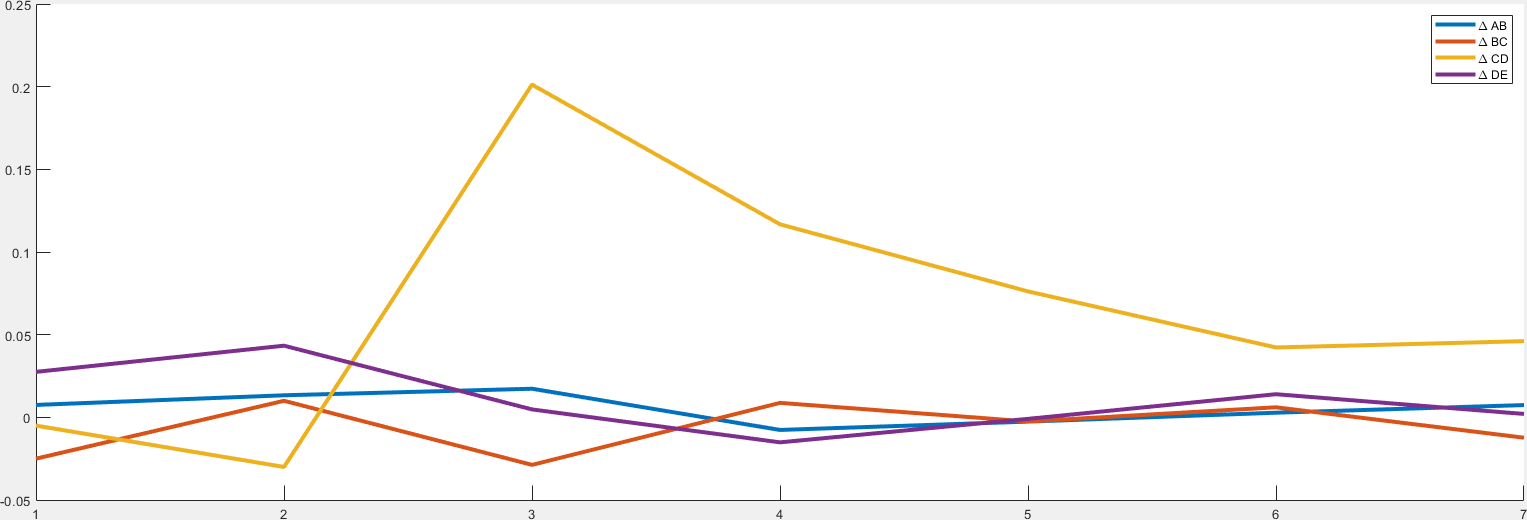
\includegraphics[width=0.9\textwidth]{images/aufgabe2} 
	\caption{Differenz} 
	\label{fig:pointdraw}
\end{figure}\\
Es ist aus dem Graph zu sehen, dass die $\overline{CD}$ hat an Zeitpunkt $t_3$ und $t_4$ deutlich geändert. 
\clearpage
\section{Aufgabe 3}
Die Runge-Kutta dient um die Differentialgleichungen zu lösen, hier soll $y' = t^2 + 2t - y + 1$ mit Anfangswert $y(0) = 0$ an der Stelle $t=0.5$ berechnet werden. Die Schrittweite $h = 0.1$.\\\\
Runge-Kutta dritter Ordnung:
\begin{align}
	y_{n+1} = & \  y_n + \frac{h}{6} (k_1 + 4k_2 + k_3) \\
	k_1 = & \  f(y_n,t_n) \\
	k_2 = & \  f(y_n + \frac{h}{2}k_1, t_n + \frac{h}{2}) \\
	k_3 = & \  f(y_n - hk_1 + 2hk_2, t_n + h) \\
	\text{mit} & \quad  f(t,y_n) = y_n'
\end{align}
Die Ergebnisse für jede Schritt:
\begin{table}[htpb]\centering
	\begin{tabular}{|c|c|c|c|c|c|c|}
		\hline
		n & 0 & 1  & 2  & 3  & 4  & 5  \\ \hline
		t &0     & 0,1    & 0,2    & 0,3    & 0,4    & 0,5    \\ \hline
		y & 0     & 0,1052 & 0,2213 & 0,3492 & 0,4897 & 0,6434 \\ \hline
	\end{tabular}
	\caption{Dritte RK Verfahren}
\end{table}\\
$y(0,5) = 0,6434$ nach Runge Kutta dritter Ordnung. \\\\
analog, Runge-Kutta vierter Ordnung: 
\begin{align} \label{2}
	y_{n+1} = & \  y_n + \frac{h}{6} (k_1 + 2k_2 +2 k_3 + k_4) \\
	k_1 = & \  f(y_n,t_n) \\
	k_2 = & \  f(y_n + \frac{h}{2}k_1, t_n + \frac{h}{2}) \\
	k_3 = & \  f(y_n + \frac{h}{2}k_2, t_n + \frac{h}{2}) \\
	k_4 = & \  f(y_n + hk_3,t_n + h) \label{3}
\end{align}
\begin{table}[htpb]\centering
	\begin{tabular}{|c|c|c|c|c|c|c|}
		\hline
		n & 0 & 1  & 2  & 3  & 4  & 5  \\ \hline
		t &0     & 0,1    & 0,2    & 0,3    & 0,4    & 0,5    \\ \hline
		y & 0     & 0,1052 & 0,2213 & 0,3492 & 0,4897 & 0,6435 \\ \hline
	\end{tabular}
	\caption{Vierte RK Verfahren}
\end{table}\\
Die Unterschied zwischen dritte und vierte Ordnung an $t = 0,5$ ist $-2,14 \cdot 10^{-5}$. Das ist sehr klein und kann in meisten Fälle ignoriert werden.  \clearpage
\section{Aufgabe 4}
Die Differentialgleichung ist von $y$ und $c$ unabhängig:
\begin{equation}\label{1}
	y' = c
\end{equation}
In dieser Aufgabe ist $y_{n+m}$ zu berücksichtigen. Nach dem Einsatz von \ref{1}:
\begin{align}
	y_{n+m} & \ = y_{n+m-1} + hc \\
	& \ = y_{n+m-2} +hc+hc \\
	 & \quad \cdots  \\
	 & \ = y_n + mhc
\end{align}
Weil $y_n$ und $c$ unkorreliert sind, lautet die Fehlerfortpflanzung
\begin{gather}
	\frac{\partial y_{n+m}}{\partial y_n} = 1 \\
	\frac{\partial y_{n+m}}{\partial c} = mh \\
	\sigma^2_{y_{m+n}} = \begin{bmatrix}
	1 & mh
	\end{bmatrix} \cdot \begin{bmatrix}
	\sigma^2_{y_n} & 0 \\
	0 & \sigma^2_{c}
	\end{bmatrix} \cdot \begin{bmatrix}
	1 \\
    mh
	\end{bmatrix} = \sigma^2_{y_n} + (mh)^2\sigma^2_{c}\\
	\sigma_{y_n} = \sqrt{\sigma^2_{y_n} + (mh)^2\sigma^2_{c}}
\end{gather}
wobei $\sigma_{y_n}$ und $\sigma_{c}$ sind die Unsicherheit von $y_n$ und $c$. \clearpage
\section{Aufgabe 5}
\subsection{a}\label{seca}
In dieser Teilaufgabe ist die Koordinaten mit Runge-Kutta Verfahren vierter Ordnung mit Schrittweite $h = \SI{100}{s}$ von $t_1 = \SI{1000}{s}$ nach $t_s = \SI{1900}{s}$ berechnet. Die Formeln sind in \ref{2} bis \ref{3}. 
\begin{table}[htbp] \centering
	\begin{tabular}{|l|l|}
		\hline
		$x$ (m)     & 1.880289566568e+07  \\ \hline
		$y$ (m)     & 1.661568254689e+07  \\ \hline
		$z$ (m)     & -4.599055621492e+06 \\ \hline
		$v_x$ (m/s) & -4.070049594214e+02  \\ \hline
		$v_y$ (m/s) & -5.159170009037e+02 \\ \hline
		$v_z$ (m/s) & -3.503303895904e+03 \\ \hline
	\end{tabular}
	\caption{Position und Geschwindigkeit an 1900s (von 1000s mit Schrittweite 100s)}
\end{table}
\subsection{b}\label{secb}
Ähnlich wie \ref{seca}, aber von $t_2 = \SI{2800}{s}$ nach $t_s$:
\begin{table}[htbp]\centering
	\begin{tabular}{|l|l|}
		\hline
		$x$ (m)     & 1.880289473488e+07  \\ \hline
		$y$ (m)     & 1.661568259796e+07  \\ \hline
		$z$ (m)     & -4.599055761960e+06 \\ \hline
		$v_x$ (m/s) & -4.070061798922e+02 \\ \hline
		$v_y$ (m/s) & -5.159183580348e+02 \\ \hline
		$v_z$ (m/s) & -3.503303232403e+03 \\ \hline
	\end{tabular}
	\caption{Position und Geschwindigkeit an 1900s (von 2800s mit Schrittweite 100s)}
\end{table}
\subsection{c}\label{secc}
\ref{seca} und \ref{secb} werden wiederholt mit Schrittweite $h = \SI{1}{s}$:
\begin{table}[htpb]\centering
	\begin{tabular}{|l|l|}
		\hline
		$x$ (m)     & 1.880289566450e+07  \\ \hline
		$y$ (m)     & 1.661568254808e+07  \\ \hline
		$z$ (m)     & -4.599055623060e+06 \\ \hline
		$v_x$ (m/s) & -4.070049591118e+02 \\ \hline
		$v_y$ (m/s) & -5.159170004552e+02 \\ \hline
		$v_z$ (m/s) & -3.503303895892e+03 \\ \hline
	\end{tabular}
	\caption{Position und Geschwindigkeit an 1900s (von 1000s mit Schrittweite 1s)}
\end{table}\clearpage
\begin{table}[htbp]\centering
	\begin{tabular}{|l|l|}
		\hline
		$x$ (m)     & 1.880289473654e+07  \\ \hline
		$y$ (m)     & 1.661568259745e+07  \\ \hline
		$z$ (m)     & -4.599055760315e+06 \\ \hline
		$v_x$ (m/s) & -4.070061799650e+02 \\ \hline
		$v_y$ (m/s) & -5.159183586592e+02 \\ \hline
		$v_z$ (m/s) & -3.503303232411e+03 \\ \hline
	\end{tabular}
	\caption{Position und Geschwindigkeit an 1900s (von 2800s mit Schrittweite 1s)}
\end{table}
\subsection{d}
In dieser Teilaufgabe werden \ref{seca}, \ref{secb} und \ref{secc} mit Runge-Kutta zweiter Ordnung statt Runge-Kutta vierter Ordnung wiederholt. 
\begin{align}
	y_{n+1} & \ = y_n + \frac{h}{2}(k_1 + k_2) \\
	k_1 & \ = f(y_n,t_n) \\
	k_2 & \ = f(y_n + hk_1, t_n + h)
\end{align}
Die Ergebnisse:
\begin{table}[htbp]\centering
	\begin{tabular}{|l|l|}
		\hline
		$x$ (m)     & 1.880296665375e+07  \\ \hline
		$y$ (m)     & 1.661559652836e+07  \\ \hline
		$z$ (m)     & -4.599185428836e+06 \\ \hline
		$v_x$ (m/s) & -4.069690930775e+02 \\ \hline
		$v_y$ (m/s) & -5.158810055287e+02 \\ \hline
		$v_z$ (m/s) & -3.503310253629e+03 \\ \hline
	\end{tabular}
	\caption{Position und Geschwindigkeit an 1900s (von 1000s mit Schrittweite 100s)(RK2)}
\end{table}\\
\begin{table}[htbp]\centering
	\begin{tabular}{|l|l|}
		\hline
		$x$ (m)     & 1.880289566450e+07  \\ \hline
		$y$ (m)     & 1.661568254808e+07  \\ \hline
		$z$ (m)     & -4.599055623060e+06 \\ \hline
		$v_x$ (m/s) & -4.070049591118e+02 \\ \hline
		$v_y$ (m/s) & -5.159170004552e+02 \\ \hline
		$v_z$ (m/s) & -3.503303895892e+03 \\ \hline
	\end{tabular}
	\caption{Position und Geschwindigkeit an 1900s (von 2800s mit Schrittweite 100s)(RK2)}
\end{table}
\clearpage
\begin{table}[htbp]\centering
	\begin{tabular}{|l|l|}
		\hline
		$x$ (m)     & 1.880289567170e+07  \\ \hline
		$y$ (m)     & 1.661568253962e+07  \\ \hline
		$z$ (m)     & -4.599055636036e+06 \\ \hline
		$v_x$ (m/s) & -4.070049555093e+02 \\ \hline
		$v_y$ (m/s) & -5.159169968526e+02 \\ \hline
		$v_z$ (m/s) & -3.503303896449e+03 \\ \hline
	\end{tabular}
	\caption{Position und Geschwindigkeit an 1900s (von 1000s mit Schrittweite 1s)(RK2)}
\end{table}
\begin{table}[htbp]\centering
	\begin{tabular}{|l|l|}
		\hline
		$x$ (m)     & 1.880289473468e+07  \\ \hline
		$y$ (m)     & 1.661568261063e+07  \\ \hline
		$z$ (m)     & -4.599055748626e+06 \\ \hline
		$v_x$ (m/s) & -4.070061827672e+02 \\ \hline
		$v_y$ (m/s) & -5.159183628987e+02 \\ \hline
		$v_z$ (m/s) & -3.503303230858e+03 \\ \hline
	\end{tabular}
	\caption{Position und Geschwindigkeit an 1900s (von 2800s mit Schrittweite 1s)(RK2)}
\end{table}
\subsection{e}
Die Differenzen zwischen den Vorwärts- und Rückwärtsintegration:
\begin{table}[htbp]\centering
	\begin{tabular}{|c|c|c|}
		\hline
						   & Schrittweite 1s & Schrittweite 100s \\ \hline
		$\Delta x$ (m)     & -0,9280 & -0,9308 \\ \hline
		$\Delta y$ (m)     & 0,0494  & 0,0511  \\ \hline
		$\Delta z$ (m)     & -0,1373 & -0,1405 \\ \hline
		$\Delta v_x$ (m/s) & -12,2085e-04 & -12,2047e-04 \\ \hline
		$\Delta v_y$ (m/s) & -13,5820e-04 & -13,5713e-04 \\ \hline
		$\Delta v_z$ (m/s) & 6,6348e-04 & 6,6350e-04 \\ \hline
	\end{tabular}
	\caption{Differenz zwischen den Vorwärts und Rückwärtsintegration}
\end{table}\\
Vorwärts- und Rückwärtsintegration auf die gleiche Position kommt unterschiedliche Ergebnisse. Die Unterschied bei Position ist ca. 1 meter und bei Geschwindigkeit ist ca. 1,9 mm/s. \\\\
Die Differenzen zwischen die Koordinaten mit \SI{1}{s} und \SI{100}{s} Schrittweite. Seh(\ref{tab:diff1}). Die Unterschied bei Position ist ca. $2,3$ mm und bei Geschwindigkeit ist ca. $5,4 \cdot 10^{-4}$ mm/s.\\\\
Die Ergebnisse von Runge-Kutta 2. Ordnung hat eine große Unterschied von der von 4. Ordnung. Wenn man die genaue Ergebnisse bekommen möchten, soll man 2. Ordnung vermeiden zu verwenden, besonders bei großem Integrationsintervall.
\begin{table}[h]\centering
	\begin{tabular}{|c|c|c|}
		\hline
		& Vorwärtsintegration & Rückwärtsintegration \\ \hline
		$\Delta x$ (m)     & 11,8633e-04 & -16.6238e-04 \\ \hline
		$\Delta y$ (m)     & -11,8876e-04  & -5.0370e-04  \\ \hline
		$\Delta z$ (m)     & -15,6822e-04 & -16,4537e-04 \\ \hline
		$\Delta v_x$ (m/s) & -3,0966e-07 & 7,2855e-07 \\ \hline
		$\Delta v_y$ (m/s) & -4,4851e-07 & 6,2440e-07 \\ \hline
		$\Delta v_z$ (m/s) & -1,1609e-08 & 7,7889e-08 \\ \hline
	\end{tabular}
	\caption{Differenz von verschiedenen Schrittweiten}
	\label{tab:diff1}
\end{table}
